% CVPR 2022 Paper Template
% based on the CVPR template provided by Ming-Ming Cheng (https://github.com/MCG-NKU/CVPR_Template)
% modified and extended by Stefan Roth (stefan.roth@NOSPAMtu-darmstadt.de)

\documentclass[10pt,twocolumn,letterpaper]{article}

%%%%%%%%% PAPER TYPE  - PLEASE UPDATE FOR FINAL VERSION
% \usepackage[review]{cvpr}      % To produce the REVIEW version
\usepackage{cvpr}              % To produce the CAMERA-READY version
%\usepackage[pagenumbers]{cvpr} % To force page numbers, e.g. for an arXiv version

% Include other packages here, before hyperref.
\usepackage{graphicx}
\usepackage{amsmath}
\usepackage{amssymb}
\usepackage{booktabs}
\usepackage{times}
\usepackage{latexsym}
\usepackage{hyperref}
\usepackage{graphicx}
\usepackage{amsmath}
\usepackage{comment}
\usepackage{placeins}
\usepackage[normalem]{ulem}
\usepackage{float}
\restylefloat{table}


% It is strongly recommended to use hyperref, especially for the review version.
% hyperref with option pagebackref eases the reviewers' job.
% Please disable hyperref *only* if you encounter grave issues, e.g. with the
% file validation for the camera-ready version.
%
% If you comment hyperref and then uncomment it, you should delete
% ReviewTempalte.aux before re-running LaTeX.
% (Or just hit 'q' on the first LaTeX run, let it finish, and you
%  should be clear).

% \usepackage[pagebackref,breaklinks,colorlinks]{hyperref}


% Support for easy cross-referencing
\usepackage[capitalize]{cleveref}
\crefname{section}{Sec.}{Secs.}
\Crefname{section}{Section}{Sections}
\Crefname{table}{Table}{Tables}
\crefname{table}{Tab.}{Tabs.}


%%%%%%%%% PAPER ID  - PLEASE UPDATE
\def\cvprPaperID{*****} % *** Enter the CVPR Paper ID here
\def\confName{CVPR}
\def\confYear{2022}

\begin{document}



%%%%%%%%% TITLE - PLEASE UPDATE
\title{Low Resolution Image Classification}


\author{Taoan Lu \qquad Tianjun Li \qquad Tiancheng Zhang \qquad Yanfu Guo \qquad Yifan Dong \\
University of Michigan, Ann Arbor\\
{\tt\small \{taoanlu, ltianjun, zhangtc, yanfuguo, spikedyf\}@umich.edu}}
% For a paper whose authors are all at the same institution,
% omit the following lines up until the closing ``}''.
% Additional authors and addresses can be added with ``\and'',
% just like the second author.
% To save space, use either the email address or home page, not both
% \and

\maketitle


%%%%%%%%% BODY TEXT
\section{Introduction}
\par The progress of the image classification is to categorize the images given into different categories based on their semantic contents in the picture. The features in the images, i.e. the image quality and resolutions, are important factors in image classification. The accuracy of image classification can be performed pretty well if the images are well depicted in a high resolution(HR) image. However, many features of the image can be missing when low resolution(LR) images compared to the high resolution images that are applied to the classifier. 

\par Therefore, such condition raises the problem on how to improve the performance when the low resolution image are applied to the image classifier. Our solution is to combine the super resolution techniques to enrich the image details of the low resolution images. Our main principle is to verify that a good Super Resolution tool can supplement the missing details in the low resolution images so that the image classification can achieve better performance.

\subsection{Background Information}
\textbf{Super Resolution: } Super Resolution(SR) is a process to obtain high-resolution from one or more low-resolution observations\cite{Nasrollahi2014}, the SR techniques mainly focus on giving more details than the given grids by increasing the pixels in per unit area. Different from the interpolation, which uses the unblurring, sharpening methods to restore the image given\cite{Nasrollahi2014}, the super resolution method, a model of the HR scene together with the imaging parameters are given to improve the quality of the output and increase the the size(the pixels per unit area)\cite{Nasrollahi2014}. During the process, the iterative back-projection, projecting on the convex sets and maximum a posterior image prediction is the way what the common SR algorithm does \cite{papathanassiou_petrou_2005}

\textbf{Image Classification: }
Image Classification has wide range of applications. Deep Convolutional Neutral Network brings great improvement in the image classification \cite{https://doi.org/10.48550/arxiv.1512.03385}. To get a great neural network training model, the network needs the degradation process that get the accuracy saturated. When considering the model to learn, it should be important to avoid the some over-fitting problem. Therefore, an easy to optimize and the enjoyable accuracy model is expected for the designed model\cite{https://doi.org/10.48550/arxiv.1512.03385}. 

\section{Approach}
Our project firstly uses several super resolution models to restore the resolution of some low resolution images, and then compare their peak signal-to-noise ratio (PSNR) performance on some test dataset. After that, we feed the resulting super resolution images into downstream classification models to check whether super resolution will increase the performance for classification. The high-level workflow of our project is shown in Figure~\ref{fig:highlevel}.
\begin{figure}
    \centering
    \includegraphics[width=\linewidth]{Workflow.png}
    \caption{High Level Architecture}
    \label{fig:highlevel}
\end{figure}


\subsection{Dataset}
Our project uses DIV2K dataset for training the super resolution models and performs super resolution tests on the Set5 dataset. DIV2K dataset is a dataset that has 800 images for training, 100 images for validation, 100 images for testing \cite{agustsson2017ntire}. Set5 dataset is widely used for testing performance of Image Super-Resolution model and only contains five images for baby, bird, butterfly, head, and woman\cite{bevilacqua2012low}. After training process, we let these baseline and advanced SR models perform SR on the PASCAL VOC2007 dataset with 20 object classes, and then feed the resulting super solution images into our downstream classification models\cite{everingham2008pascal}. In the VOC2007 dataset, there are 5000 images for trainval set and 4952 images for the test set. Since the VOC2007 dataset only has high resolution images, we follow other paper's method to first resize the images to smaller scales\cite{wu2019unsupervised}, and then use these resized images as our lower resolution image dataset. 

\subsection{Super Resolution}

\subsubsection{Model}
Our models in the super resolution part are two baselines: 1) bicubic Interpolation, 2) Super-resolution convolution neural network (SRCNN), and one advanced model: 3) SwinIR.

{\bf Bicubic Interpolation: }Bicubic interpolation is a method for interpolating data points as an extension of cubic interpolation and is often widely used in image processing. The algorithm we use in this project is called bicubic convolution algorithm where the kernel used in the project us designed as:
\begin{figure}[h]
    \centering
    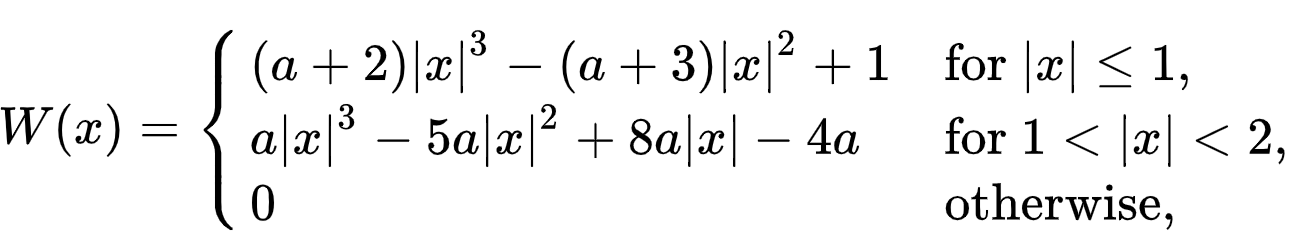
\includegraphics[width=\linewidth]{bicubic.png}
\end{figure}
By applying the kernel to the image, a prediction of the point $p(x,y)$ can be calculated as with: 
\begin{figure}[h]
    \centering
    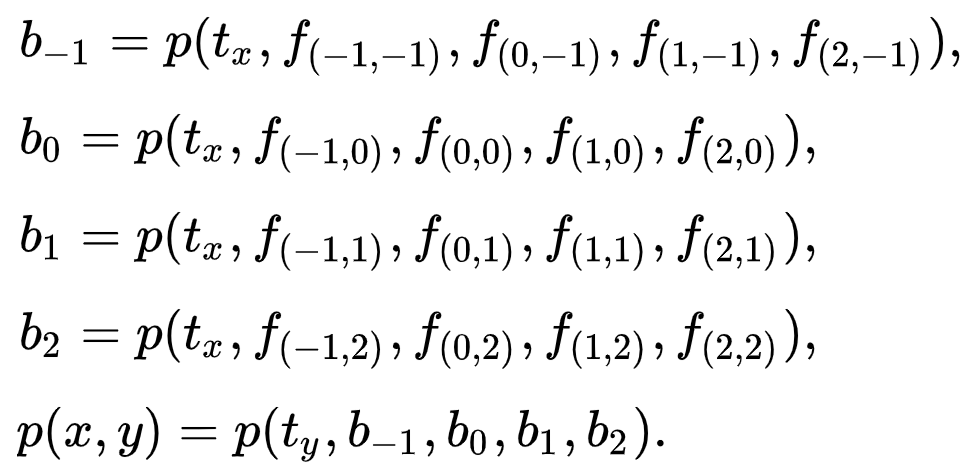
\includegraphics[width=\linewidth]{bicubic2.png}
\end{figure}

{\bf SRCNN: }Super-resolution convolution neural network (SRCNN) is a deep convolution neural network that learns end-to-end mapping of low resolution to high resolution images\cite{dong2015image}. SRCCN's processes consists of patch extraction and representation, non-linear mapping, reconstruction. For the patch extraction part, the first layer $F_1(Y) = max (0, W_1 \ast Y + B_1)$, where $W_1$ and $B_1$ are respectively the filters and biases, and $\ast$ represents the convolution operation. For the non-linear mapping part, the second layer is $F_2(Y) = max (0, W_2 \ast F_1(Y) + B_2)$, where $W_2$ and $B_2$ are respectively the filters and biases. For the reconstruction part, the third layer is $F(Y) = W_3 * F_2(Y) + B_3$, where W still stands for filters and B stands for biases. Its architecture is visualized in figure~\ref{fig:srcnn}.

\begin{figure}[h]
    \centering
    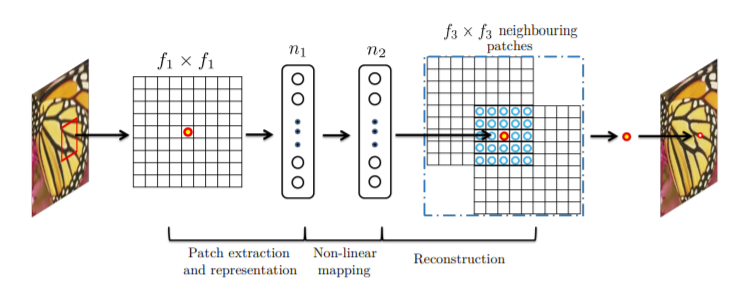
\includegraphics[width=\linewidth]{SRCNN.png}
    \caption{SRCNN Architecture\cite{dong2015image}}
    \label{fig:srcnn}
\end{figure}

{\bf SwinIR: } SwinIR is a model based on Swin Transformer and has three parts, which are respectively shallow feature
extraction, deep feature extraction and high-quality image
reconstruction modules\cite{liang2021swinir}. For shallow feature extraction, a 3 $\times$ 3 convolutional layer is used. For deep feature extraction, several connected residual Swin Transformer blocks (RSTB) and a 3 $\times$ 3 convolutional layer are used. As for the reconstruction process, it is obtained by aggregating the shallow and deep features. The loss function for image super resolution is $\mathcal{L}=\left\|I_{R H Q}-I_{H Q}\right\|_{1}$, where $I_{RHQ}$ is obtained by taking the low quality image as the input of SwinIR,
$I_{HQ}$ is the corresponding ground-truth high quality image. Its architecture is visualized in figure\ref{fig:swinir}.

\begin{figure}[h]
    \centering
    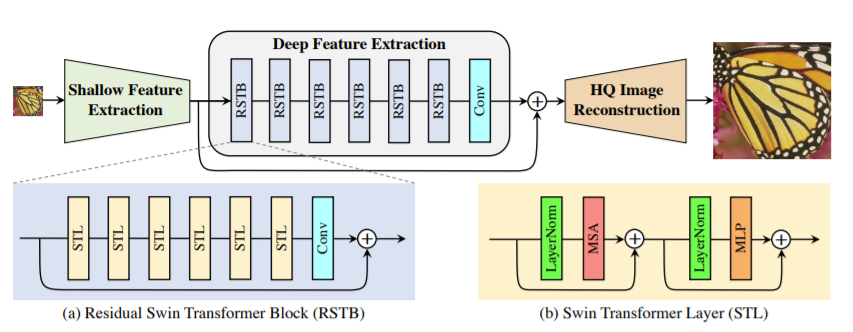
\includegraphics[width=\linewidth]{swinir.png}
    \caption{SwinIR Architecture\cite{liang2021swinir}}
    \label{fig:swinir}
\end{figure}

\subsubsection{Metric}
{\bf PSNR:} Peak signal-to-noise ratio (PSNR) is an expression for the ratio between the maximum possible value (power) of a signal and the power of distorting noise that affects the quality of its representation. Specifically, $P S N R=20 \log _{10}\left(\frac{\rm{M A X}_{f}}{\sqrt{\rm{M S E}}}\right)$ where $\rm{M S E}=\frac{1}{m\cdot n} \sum_{0}^{m-1} \sum_{0}^{n-1}\|f(i, j)-g(i, j)\|^{2}$. In the above equations, f represents the matrix data of our original image, g represents the matrix data of our degraded image in question, m represents the numbers of rows of pixels of the images, n represents the number of columns of pixels of the image. The larger the PSNR is, the higher quality the image has.

\subsection{Classification}
For classification task, we use Resnet-50 to train, and Mean Average Precision (mAP) to evaluate the performance.

\subsubsection{Model}
{\bf Resnet-50: }ResNet represents for residual networks. It is a classic neural network used for computer vision tasks. ResNet-50 is a variant of ResNet model which has 48 Convolution layers along with 1 MaxPool and 1 Average Pool layer. Our project applies ResNet-50 for classification.



\begin{figure*}[h]
\centering
    \begin{subfigure}{0.18\textwidth}
        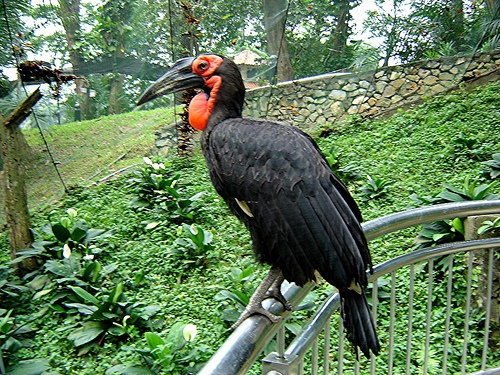
\includegraphics[width=1\linewidth]{000057.jpg} 
        \caption{Original image}
        \label{fig:subim1}
    \end{subfigure}
    \begin{subfigure}{0.18\textwidth}
        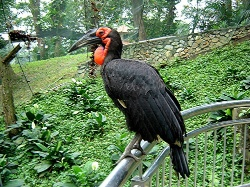
\includegraphics[width=1\linewidth]{000057-lr.jpg}
        \caption{Low resolution image}
        \label{fig:subim2}
    \end{subfigure}
    \begin{subfigure}{0.18\textwidth}
        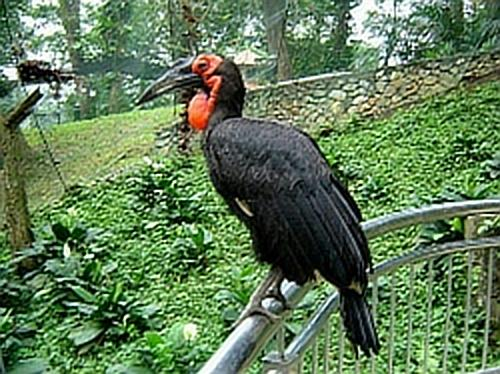
\includegraphics[width=1\linewidth]{000057-sr.jpg}
        \caption{SRCNN}
        \label{fig:subim3}
    \end{subfigure}
    \begin{subfigure}{0.18\textwidth}
        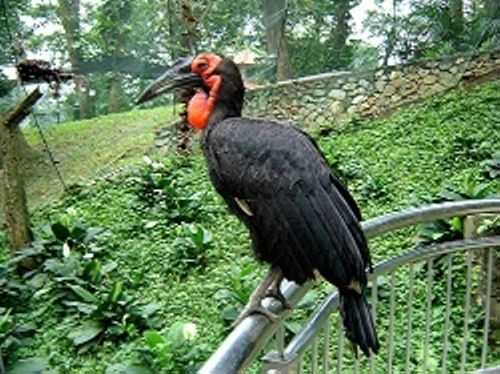
\includegraphics[width=1\linewidth]{000057-bi.jpg}
        \caption{Bicubic Interpolation}
        \label{fig:subim4}
    \end{subfigure}
    \begin{subfigure}{0.18\textwidth}
        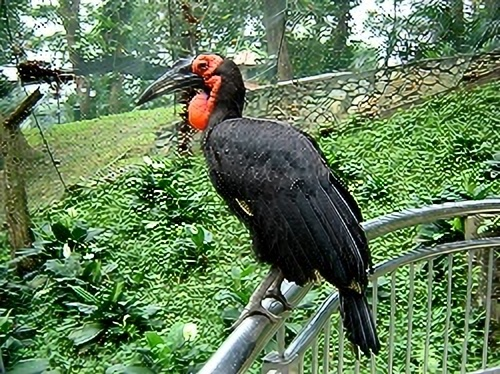
\includegraphics[width=1\linewidth]{000057-sw.jpg}
        \caption{SwinIR}
        \label{fig:subim5}
    \end{subfigure}
\caption{Visual comparison of SR methods on a test image}
\label{fig:comparison}
\end{figure*}



\begin{figure*}[h]
\centering
    \begin{subfigure}{0.18\textwidth}
        \includegraphics[width=1\linewidth]{heatmap_LR.png} 
        \caption{Overlayed Heatmap of Low Resonlution Pictures}
        \label{fig:h1}
    \end{subfigure}
    \begin{subfigure}{0.18\textwidth}
        \includegraphics[width=1\linewidth]{heat_LR.PNG}
        \caption{Heatmap of Low Resonlution Pictures}
        \label{fig:h2}
    \end{subfigure}
    \begin{subfigure}{0.18\textwidth}
        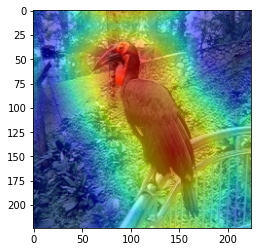
\includegraphics[width=1\linewidth]{heatmap_sw.png}
        \caption{Overlayed Heatmap of SwinIR result}
        \label{fig:h3}
    \end{subfigure}
    \begin{subfigure}{0.18\textwidth}
        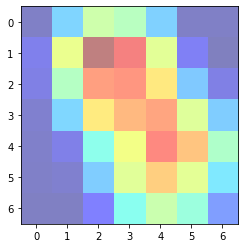
\includegraphics[width=1\linewidth]{heat_sw.png}
        \caption{Heatmap of SwinIR result}
        \label{fig:h4}
    \end{subfigure}
\caption{Heatmap on a test image}
\label{fig:heatmap}
\end{figure*}

\subsubsection{Metric}
{\bf Mean Average Precision (mAP): }  For object detection, mAP is widely used as an evaluation metric. Rather than taking the average of precision, mAP is average of average precision, where average precision(AP) is the area under the precision-recall curve. Precision and recall are respectively calculated by $\rm{Precision} = \frac{TP}{TP + FP}$, $\rm{Recall} = \frac{TP}{TP + FN}$.

\section{Experiments}
{\bf Super Resolution:} For the super resolution part, we trained, tested, and compared three models: 1) Bicubic, 2) SRCNN, 3) SwinIR. 

Bicubic performs data interpolation on the low resolution images and generates high resolution images accordingly. So for the Bicubic method, we just feed in the test dataset Set5 into it and calculate its performance. For SRCNN and SwinIR, we trained the two deep neural networks on dataset DIV2k, and tested the trained models' performance on the Set5 dataset. For bicubic method, the coefficient $a$ used in the process is 0.5. The SRCNN model use a batch size of 4, the channel of the feature extraction are 64 and 32, and the kernel size are set as 9 and 5. The best performing parameters for SwinIR that we used are: the RSTB number set to default 6, the STL number set to default 6, window size set to 8, channel number set to 180, and attention head number set to 6. 

We used PSNR (peak signal-to-noise ratio) to measure and compare the performance of our three models. This metric measures the image enhancement quality of the high resolution images generated from the low resolution ones by the SR models. The average PNSR results of the three trained models Bicubic, SRCNN, and SwinIR are summarized in table \ref{tab:PSNR}. We can see that the SwinIR model outperforms the two baseline models--SRCNN and Bicubic to a great extent.

\begin{table}[htbp!]
\centering
\begin{minipage}[htbp!]{0.5\textwidth}
\centering
\scalebox{0.7}{
\begin{tabular}{ p{3cm}||p{2cm}p{2cm}p{2cm} }

 & SwinIR&Bicubic &SRCNN\\
\hline
\hline
Average PSNR & 36.15 & 28.69 &  31.73\\
\end{tabular}}
\end{minipage}
\caption{Average PSNR of Different Super Resolution Technique}
\label{tab:PSNR}
\end{table}

{\bf Downstream Classification:} In this part, we use Mean Average Precision (mAP) to measure the overall success of the multi-label classification results. We first train a 3-conv-layer CNN based on 442 assignment. However, the test mAP is only 0.1796, which can hardly be used. Therefore, we train a Resnet-50 model on VOC2007 dataset and use it to test the performance of our SwinIR model. To be specific, the trained Resnet-50 model is a multi-label image classifier and it takes 5 test sets as input: the original pictures in VOC2007 test set, the low resolution pictures, the SwinIR results, the SRCNN results and the Bicubic Interpolation results. Figure \ref{fig:comparison} shows the visual comparison of those 5 sets. We can see that the resolution has been improved to a great extent by using SwinIR. Table \ref{tab:mean} shows the quantitative comparisons among those 5 test sets and  Table \ref{tab:all} shows the Average Precision(AP) for each class. 
\par

\begin{table}[h!]
\centering
\begin{minipage}[htbp!]{0.5\textwidth}
\centering
\scalebox{0.5}{
\begin{tabular}{ p{2cm}||p{2cm}p{2cm}p{2cm}p{2cm}p{2cm}  }

 & Original Pictures&Low-Resolution Pictures &SRCNN Result&Bicubic Result&SwinIR Result\\
\hline
\hline
Mean Average Precision & 0.9091 & 0.9050 & 0.8907 & 0.8998 & 0.9021 \\
\end{tabular}}
\end{minipage}
\caption{Mean Average Precision under Different Test Set}
\label{tab:mean}
\end{table}

\begin{table*}[h!]
\centering
\begin{minipage}{0.8\textwidth}
\centering
\begin{tabular}{ p{2cm}||p{2cm}p{2cm}p{2cm}p{2cm}p{2cm}  }
 Average Precision & Original Pictures&Low-Resolution Pictures &SRCNN Result&Bicubic Result&SwinIR Result\\
\hline
\hline
 Aeroplane   & 0.9857   & 0.9815    & 0.9794    & 0.9761    & 0.9810\\
 Bicycle     & 0.9495   & 0.9530    & 0.9323    & 0.9400    & 0.9439\\
 Bird        & 0.9492   & 0.9494    & 0.9453    & 0.9493    & 0.9451\\
 Boat        & 0.9457   & 0.9523    & 0.9430    & 0.9482    & 0.9545\\
 Bottle      & 0.6354   & 0.6068    & 0.5760    & 0.5853    & 0.6076\\
 Bus         & 0.9320   & 0.9260    & 0.9022    & 0.9078    & 0.9252\\
 Car         & 0.9354   & 0.9311    & 0.9280    & 0.9321    & 0.9313\\
 Cat         & 0.9182   & 0.9006    & 0.8986    & 0.8967    & 0.9051\\
 Chair       & 0.7546   & 0.7627    & 0.7636    & 0.7676    & 0.7563\\
 Cow         & 0.8726   & 0.8560    & 0.8327    & 0.8324    & 0.8594\\ 
 Dining Table& 0.7776   & 0.7916    & 0.7564    & 0.7732    & 0.7557\\
 Dog         & 0.9322   & 0.9362    & 0.9061    & 0.9409    & 0.9198\\
 Horse       & 0.9676   & 0.9635    & 0.9569    & 0.9585    & 0.9632\\
 Motor Bike  & 0.9006   & 0.8898    & 0.8717    & 0.8813    & 0.8866\\
 Person      & 0.9676   & 0.9637    & 0.9569    & 0.9605    & 0.9617\\
 Potted Plane& 0.7412   & 0.7472    & 0.7355    & 0.7392    & 0.7589\\
 Sheep       & 0.9069   & 0.8977    & 0.8735    & 0.8921    & 0.8880\\
 Sofa        & 0.6550   & 0.6848    & 0.7005    & 0.6814    & 0.6864\\
 Train       & 0.9817   & 0.9760    & 0.9726    & 0.9712    & 0.9759\\
 Tv Monitor  & 0.8230   & 0.8172    & 0.8181    & 0.8252    & 0.8311\\
\end{tabular} 

\end{minipage}
\caption{Average Precision of Different Classification under Different Test Set}
\label{tab:all}
\end{table*}

As one can see, when tested on the original test set of the VOC2007, we reach a mAP of 0.9091, which can also show that the performance of the model is great. The mAP for low resolution test set is 0.9050, higher than 0.8907 for SRCNN, 0.8998 for Bicubic and 0.9021 for SwinIR. It is counter-intuitive that the mAP for super resolution results are lower. It means that the SwinIR is not helping the classification. One possible explanation is that some useful features in the low resolution image are lost. SwinIR model may add too many artificial details. 

\par To help figure out the reason, we try Class Activation Mappings (CAM) which overlay a heatmap over the original image to show us where our model focus on. Figure \ref{fig:heatmap} shows the focus of the final convnet layer when the input is the low resolution picture and SwinIR result. We can see that those two heatmaps are slightly different from each other, especially in the bird's head and body regions. Further analysis is still needed to determine the exact reason of why SwinIR cannot help the classification.



\section{Implementation}
For the super resolution part, we implement the down sample code on our own. We then refer to the SwinIR network model from the following link \href{https://github.com/JingyunLiang/SwinIR}{(https://github.com/JingyunLiang/SwinIR)}. We modify the test and picture generation function to our needs. For the baselines super resolution method. The bicubic is implemented by ourselves based on the algorithm and the SRCNN makes reference to the following link \href{https://github.com/Mirwaisse/SRCNN}{(https://github.com/Mirwaisse/SRCNN)}. The dataset for train and test are modified and the parameters including the batch size and the number of training epoch are adjusted to achieve better performance. \par
For the classification part, we refer to a residual network model from the following link \href{https://github.com/lyz04551/voc2007_classification_pytorch}{(https://github.com/lyz04551/voc2007{\_}classification{\_}pytorch)}. We add some functions calculating the average precision on all classes and the mean average precision. We redesign and simplify the randomnized data loader because the focus of the project is not on the image classification. We also add code for the heatmap generation to visualize the output of the model applied by following this tutorial \href{http://www.snappishproductions.com/blog/2018/01/03/class-activation-mapping-in-pytorch.html.html}{(http://www.snappishproductions.com/blog/2018/01/03/class-activation-mapping-in-pytorch.html.html)}.

%%%%%%%%% REFERENCES
{\small
\bibliographystyle{ieee_fullname}
\bibliography{egbib}
}


\end{document}
